\documentclass{article}
\usepackage[utf8]{inputenc}
\usepackage{amsmath}
\usepackage{graphicx}
\usepackage{listings}
\usepackage{geometry}
\usepackage{hyperref}
\usepackage{float}

\geometry{a4paper, margin=1in}

\title{Relatório do Exercício de Aplicação do PCA}
\author{Eduardo Henrique Basilio de Carvalho}
\date{\today}

\begin{document}

\maketitle

\section{Objetivo}
Aplicar PCA (Principal Component Analysis) para extrair características mais relevantes e reduzir a dimensionalidade dos dados de imagens de dígitos manuscritos (MNIST). O intuito é manter o máximo possível da variância da informação original, visando acelerar o treinamento dos modelos de classificação.

\section{Exercício}

\subsection{1. Carregar o conjunto de dados MNIST e 2. Visualizar algumas imagens}
O conjunto de dados MNIST foi carregado e algumas imagens foram visualizadas para entender o formato dos dados.

\begin{figure}[H]
\centering
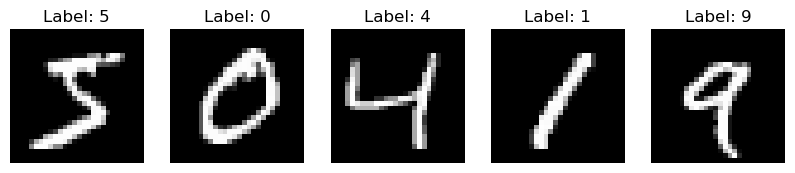
\includegraphics[width=0.8\textwidth]{digits.png}
\caption{Visualização de alguns dígitos do MNIST}
\end{figure}

\subsection{3. Aplicar PCA com diferentes números de componentes e 4. Extrair a variância explicada}
O PCA foi aplicado com 10, 30, 50 e 100 componentes. A variância explicada por cada um é apresentada abaixo.

\textbf{Variância Explicada:}
\begin{itemize}
    \item Com 10 componentes: 48.92\%
    \item Com 30 componentes: 73.16\%
    \item Com 50 componentes: 82.54\%
    \item Com 100 componentes: 91.46\%
\end{itemize}

\subsection{5. Treinar classificador e comparar acurácia}
Um classificador SVM foi treinado com os dados originais (784 features) e com os dados reduzidos pelo PCA. A acurácia e o tempo de treinamento foram comparados.

\textbf{Resultados com Dados Originais:}
\begin{itemize}
    \item Acurácia: 0.98 $\pm$ 0.00
    \item Tempo: 763.85 segundos
\end{itemize}

\textbf{Resultados com Dados Reduzidos pelo PCA:}
\begin{itemize}
    \item 10 Componentes: Acurácia 0.94 $\pm$ 0.00, Tempo 45.15s
    \item 30 Componentes: Acurácia 0.98 $\pm$ 0.00, Tempo 61.61s
    \item 50 Componentes: Acurácia 0.98 $\pm$ 0.00, Tempo 100.34s
    \item 100 Componentes: Acurácia 0.98 $\pm$ 0.00, Tempo 162.72s
\end{itemize}

\textbf{Sumário dos Resultados:}
\begin{table}[H]
\centering
\begin{tabular}{|l|c|c|r|}
\hline
Dados                 & Acurácia Média & Std Acurácia & Tempo (s) \\ \hline
Original              & 0.977971       & 0.002110     & 763.85    \\ \hline
PCA (10 componentes)  & 0.935286       & 0.002889     & 45.15     \\ \hline
PCA (30 componentes)  & 0.979843       & 0.001363     & 61.61     \\ \hline
PCA (50 componentes)  & 0.982414       & 0.001669     & 100.34    \\ \hline
PCA (100 componentes) & 0.982314       & 0.001727     & 162.72    \\ \hline
\end{tabular}
\caption{Comparação de acurácia e tempo de treinamento.}
\end{table}

\subsection{6. Visualizar dados em 2D com as duas primeiras componentes principais}
Os dados foram projetados nas duas primeiras componentes principais para visualização da separação entre classes.

\begin{figure}[H]
\centering
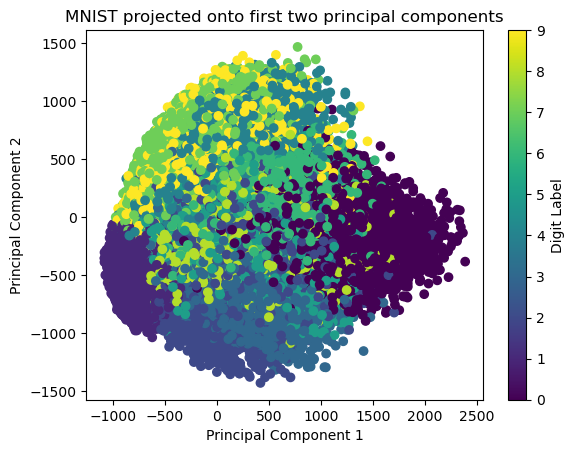
\includegraphics[width=0.8\textwidth]{2PCs.png}
\caption{Dados MNIST projetados nas duas primeiras componentes principais.}
\label{fig:pca_2d}
\end{figure}

A Figura \ref{fig:pca_2d} mostra que os dois compoentes principais não são suficientes para separar, com segurança, as classes de dígitos manuscritos. No entanto, é possível observar alguma separação entre algumas classes.

\subsection{7. Discussão}
\begin{itemize}
    \item \textbf{Qual o melhor número de componentes?} Analisando a tabela de sumário, PCA com 50 componentes parece ser o melhor equilíbrio. Ele atinge uma acurácia média ligeiramente superior à dos dados originais (0.9824 vs 0.9780) e aos 100 componentes (0.9823), com um tempo de treinamento significativamente menor (100.34s vs 763.85s para original, e vs 162.72s para 100 componentes). PCA com 30 componentes também apresenta uma acurácia comparável (0.9798) com um tempo ainda menor (61.61s), sendo uma alternativa muito boa se a velocidade for crítica. 10 componentes resultam em uma queda considerável na acurácia (0.9353).
    \item \textbf{Quanta variância você perde?}
        \begin{itemize}
            \item Com 10 componentes: Perde-se 100\% - 48.92\% = 51.08\% da variância.
            \item Com 30 componentes: Perde-se 100\% - 73.16\% = 26.84\% da variância.
            \item Com 50 componentes: Perde-se 100\% - 82.54\% = 17.46\% da variância.
            \item Com 100 componentes: Perde-se 100\% - 91.46\% = 8.54\% da variância.
        \end{itemize}
    \item \textbf{Qual o impacto no tempo e na acurácia?} A redução de dimensionalidade com PCA teve um impacto drástico na redução do tempo de treinamento. Com 50 componentes, o tempo foi reduzido em aproximadamente 87\% (de 763.85s para 100.34s) em comparação com os dados originais, enquanto a acurácia ligeiramente melhorou. Mesmo com 100 componentes, o tempo foi reduzido em cerca de 79\% com acurácia similar. Com 10 componentes, a redução de tempo foi a maior (cerca de 94\%), mas houve uma queda na acurácia de aproximadamente 4.4\%.
\end{itemize}

\section{Perguntas para reflexão}
\begin{itemize}
    \item \textbf{O PCA preserva a interpretabilidade das features originais?} Não, o PCA não preserva a interpretabilidade das features originais. As componentes principais são combinações lineares das features originais e, geralmente, não correspondem diretamente a nenhuma das features originais de forma intuitiva. Elas são ordenadas pela quantidade de variância que explicam, mas sua interpretação direta em termos do problema original (pixels específicos em uma imagem, por exemplo) é perdida.
    \item \textbf{É possível que a acurácia melhore mesmo com menos dimensões? Por quê?} Sim, é possível. Isso pode ocorrer por algumas razões:
        \begin{itemize}
            \item \textbf{Redução de Ruído:} O PCA pode ajudar a remover ruído e redundância dos dados, mantendo as features mais informativas. Dimensões com pouca variância (que são descartadas) podem conter mais ruído do que sinal útil para a classificação.
            \item \textbf{Mitigação da Maldição da Dimensionalidade:} Com muitas features, alguns algoritmos de aprendizado de máquina podem sofrer com a maldição da dimensionalidade, onde o espaço de features se torna tão esparso que os dados de treinamento não conseguem generalizar bem. Reduzir as dimensões pode ajudar o modelo a generalizar melhor.
            \item \textbf{Overfitting:} Modelos treinados em dados de alta dimensionalidade podem ser mais propensos a overfitting (ajustar-se demais aos dados de treinamento, incluindo o ruído). A redução de dimensionalidade pode atuar como uma forma de regularização, levando a um modelo mais robusto.
        \end{itemize}
        No presente exercício, observamos uma ligeira melhoria na acurácia com 50 componentes em comparação com os dados originais.
    \item \textbf{O PCA é um método supervisionado ou não supervisionado?} O PCA é um método \textbf{não supervisionado}. Ele analisa apenas as features (X) para encontrar as direções de maior variância, sem utilizar os rótulos das classes (y) durante o processo de cálculo das componentes principais.
\end{itemize}

\section{Conclusão}
A aplicação do PCA no conjunto de dados MNIST demonstrou ser eficaz na redução da dimensionalidade, resultando em uma diminuição significativa no tempo de treinamento do classificador SVM. Com 50 componentes principais, foi possível alcançar uma acurácia ligeiramente superior à obtida com todas as 784 features, enquanto se reteve 82.54\% da variância original e se reduziu o tempo de treinamento em aproximadamente 87\%. Isso ilustra o potencial do PCA para otimizar modelos de aprendizado de máquina em conjuntos de dados de alta dimensionalidade.

\end{document}